\documentclass[12pt,a4paper,bibliography=totocnumbered,listof=totocnumbered]{article}
% u.U. muss Koma-Skript Package ueber MikTeX deinstalliert und neu installiert werden
% Hilft das nicht, so sollte statt scrartcl die Dokumentenklasse article verwendet werden
\usepackage[backend=bibtex,style=alphabetic]{biblatex}
\usepackage[ngerman]{babel}
\usepackage[utf8]{inputenc}
\usepackage{ifthen}
\usepackage{xargs}
\usepackage{amsmath}
\usepackage{amsfonts}
\usepackage{amssymb}
\usepackage{graphicx}
\usepackage{fancyhdr}
\usepackage{tabularx}
\usepackage{geometry}
\usepackage{setspace}
\usepackage[right]{eurosym}
\usepackage[printonlyused]{acronym}
\usepackage{subfig}
\usepackage{floatflt}
\usepackage[usenames,dvipsnames]{color}
\usepackage{colortbl}
\usepackage{paralist}
\usepackage{array}
\usepackage{titlesec}
\usepackage{parskip}
\usepackage[right]{eurosym}
\usepackage[subfigure,titles]{tocloft}
\usepackage[pdfpagelabels=true]{hyperref}

\usepackage{listings}
\lstset{basicstyle=\footnotesize, captionpos=b, breaklines=true, showstringspaces=false, tabsize=2, frame=lines, numbers=left, numberstyle=\tiny, xleftmargin=2em, framexleftmargin=2em}
\makeatletter
\def\l@lstlisting#1#2{\@dottedtocline{1}{0em}{1em}{\hspace{1,5em} Lst. #1}{#2}}
\makeatother

\geometry{a4paper, top=27mm, left=20mm, right=20mm, bottom=35mm, headsep=10mm, footskip=12mm}

\definecolor{javared}{rgb}{0.6,0,0} % for strings
\definecolor{javagreen}{rgb}{0.25,0.5,0.35} % comments
\definecolor{javapurple}{rgb}{0.5,0,0.35} % keywords
\definecolor{javadocblue}{rgb}{0.25,0.35,0.75} % javadoc
\definecolor{gray}{rgb}{0.6,0.6,0.6}
 
\lstset{language=Java,
basicstyle=\ttfamily\footnotesize,
keywordstyle=\color{javapurple}\bfseries,
stringstyle=\color{javared},
commentstyle=\color{javagreen}\itshape\bfseries,
morecomment=[s][\color{javadocblue}]{/**}{*/},
numbers=left,
numberstyle=\tiny\color{gray},
stepnumber=1,
numbersep=10pt,
tabsize=3,
showspaces=false,
showstringspaces=false}
% Kopf- und Fusszeile
\renewcommand{\sectionmark}[1]{\markright{#1}}
\renewcommand{\leftmark}{\rightmark}
\pagestyle{fancy}
\lhead{}
\chead{}
\rhead{\thesection\space\contentsname}
\lfoot{}
\cfoot{}
\rfoot{\ \linebreak Seite \thepage}
\renewcommand{\headrulewidth}{0.4pt}
\renewcommand{\footrulewidth}{0.4pt}

% Vorspann
\renewcommand{\thesection}{\Roman{section}}
\renewcommand{\theHsection}{\Roman{section}}
\pagenumbering{Roman}

\newcommand{\folgen}[1]{
\ensuremath
#1
}

\newcommandx{\student}[3][]{
	\def\studentName{#1}%
	\def\studentMatnr{#2}%
	\def\studentStudiengang{#3}%
}


\newcommandx{\MyTitelseite}[8][]{
\thispagestyle{empty}

\includegraphics[scale=0.2]{pics/oth-logo.png}\hfill
\IfFileExists{#1}{\includegraphics[scale=0.5]{#1}}{}
\begin{center}
\ifthenelse{\equal{#2}{2}}{ % then
	\vspace*{2cm}
	\Large
	\textbf{Ostbayerische Technische Hochschule Regensburg}\\
	\textbf{Fakultät für Informatik und Mathematik}\\
	\vspace*{2cm}
	\Huge
	\textbf{#3}\\[1em]
	\large
	Zur Erlangung des akademischen Grades des\\
	\ifthenelse{\equal{#3}{Bachelorarbeit}}{Bachelor of Science (B.Sc.)}{Master of Science (M.Sc.)}\\
	\vspace*{1cm}
	\Large
	\textbf{#4}\\
}{ % else
	\vspace*{1cm}
	\Large
	\textbf{#4}\\
	\vspace*{2cm}
	\large
	An der Fakultät für Informatik und Mathematik der\\
	Ostbayerischen Technischen Hochschule Regensburg\\
	im Studiengang\\
	\studentStudiengang\\[2em]
	eingereichte\\
	\vspace*{1cm}
	\Large
	\textbf{#3}\\[2em]
	\large
	zur Erlangung des akademischen Grades des\\
	\ifthenelse{\equal{#3}{Bachelorarbeit}}{Bachelor of Science (B.Sc.)}{Master of Science (M.Sc.)}
	\vspace*{1cm}
	\Large
}
	\vfill
	\normalsize
	%\newcolumntype{x}[1]{>{\raggedleft\arraybackslash\hspace{0pt}}p{#1}}
	\begin{tabular}{rl}%{6cm}p{7.5cm}}
	    \rule{0mm}{1ex}\textbf{Vorgelegt von:} & \studentName \\
		\rule{0mm}{1ex}\textbf{Matrikelnummer:} & \hspace*{-0.5em}\begin{tabular}[t]{r}\studentMatnr\end{tabular} \\ 
		\ifthenelse{\equal{#2}{1}}{~\\}{\rule{0mm}{1ex}\textbf{Studiengang:} & \studentStudiengang \\[2em]}
		\rule{0mm}{1ex}\textbf{Erstgutachter:} & #5 \\ 
		\rule{0mm}{1ex}\textbf{Zweitgutachter:} & #6 \\[2em]
		\rule{0mm}{1ex}\textbf{Abgabedatum:} & #7 \\ 
	\end{tabular} 
\end{center}
\pagebreak
}

\newsavebox\mybox
\savebox\mybox{%
  \tikz{
    \draw[ultra thick,red] (-4pt,-4pt) -- (4pt,4pt);
    \draw[ultra thick,red] (-4pt,4pt) -- (4pt,-4pt);
  }%
}  

\newcommand{\TopAlign}[1]{\adjustbox{valign=t}{#1}}
\newcolumntype{T}{>{\collectcell{\TopAlign}}c<{\endcollectcell}}



\forestset{
  upsideTria/.style={
    node format={
      \noexpand\node [
      draw,
      shape=regular polygon,
      regular polygon sides=3,
      inner sep=0pt,
      outer sep=0pt,
      \forestoption{node options},
      anchor=\forestoption{anchor}
      ]
      (\forestoption{name}) {\foresteoption{content format}};
    },
    child anchor=parent,
  },
  downsideTria/.style={
     node format={
      \noexpand\node [
      draw,
      shape=regular polygon,
      regular polygon sides=3,
      shape border rotate=180,
	  inner sep=0pt,
      outer sep=0pt,
      \forestoption{node options},
      anchor=\forestoption{anchor}
      ]
      (\forestoption{name}) {\foresteoption{content format}};
    },
    child anchor=parent, 
  },
  downsideTriaTerm/.style={
     node format={
      \noexpand\node [
      draw,
      shape=regular polygon,
      regular polygon sides=3,
      shape border rotate=180,
	  inner sep=0pt,
	  outer sep=0pt,
	  fill=green,
      \forestoption{node options},
      anchor=\forestoption{anchor}
      ]
      (\forestoption{name}) {\foresteoption{content format}};
    },
    child anchor=parent, 
  },
  upsideTriaTerm/.style={
    node format={
      \noexpand\node [
      draw,
      shape=regular polygon,
      regular polygon sides=3,
      inner sep=0pt,
      outer sep=0pt,
	  fill=green,
      \forestoption{node options},
      anchor=\forestoption{anchor}
      ]
      (\forestoption{name}) {\foresteoption{content format}};
    },
    child anchor=parent,
  },
  upsideTriaYellow/.style={
    node format={
      \noexpand\node [
      draw,
      shape=regular polygon,
      regular polygon sides=3,
      inner sep=0pt,
      outer sep=0pt,
	  fill=yellow,
      \forestoption{node options},
      anchor=\forestoption{anchor}
      ]
      (\forestoption{name}) {\foresteoption{content format}};
    },
    child anchor=parent,
  },
  downsideTriaYellow/.style={
     node format={
      \noexpand\node [
      draw,
      shape=regular polygon,
      regular polygon sides=3,
      shape border rotate=180,
	  inner sep=0pt,
	  outer sep=0pt,
	  fill=yellow,
      \forestoption{node options},
      anchor=\forestoption{anchor}
      ]
      (\forestoption{name}) {\foresteoption{content format}};
    },
	child anchor=parent,
  }
}

\tikzset{
myedge/.style={
  decoration={
   markings,
   mark=at position 0.5 with \node {\usebox\mybox};
  },
  postaction=decorate
  }
}
\addbibresource{literatur.bib}


\begin{document}


% ----------------------------------------------------------------------------------------------------------
% Titelseite
% ----------------------------------------------------------------------------------------------------------
\newcommand{\studierenderName}{Korbinian Federholzner}
\student{\studierenderName}		% Studierender
{3114621}						% Matrikelnummer
{Techniche Informatik}			% Studiengang

\MyTitelseite{}	% Optionales Logo des extern betreuenden Unternehmens
{1}								% Style der Titelseite (1 oder 2)
{Bachelorarbeit}				% Typ der Abschlussarbeit (\in {Bachelorarbeit, Masterarbeit})
{Entwicklung einer künstlichen Intelligenz für Brettspiele und deren Anbindung an eine Touch-Hardware über mobiele Endgeräte}				% Thema der Arbeit						
{Prof.\ Dr.\ Carsten Kern}		% Betreuer
{Prof.\ Dr. \ Daniel Jobst}	% Zweitgutachter
{31.08.\the\year}				% Abgabedatum

\thispagestyle{empty}
~\pagebreak

\setcounter{page}{1} 

% ----------------------------------------------------------------------------------------------------------
% Eigensctändigkeitserklaerung
% ----------------------------------------------------------------------------------------------------------
\thispagestyle{empty}
\section*{Erklärung zur Bachelorarbeit}

\bigskip
\bigskip 
\bigskip 

\begin{enumerate}
    \item Mir ist bekannt, dass dieses Exemplar der Abschlussarbeit als Prüfungsleistung in das Eigentum der Ostbayerischen Technischen Hochschule Regensburg übergeht.
    \item Ich erkläre hiermit, dass ich diese Abschlussarbeit selbständig verfasst, noch nicht anderweitig für Prüfungszwecke vorgelegt, keine anderen als die angegebenen Quellen und Hilfsmittel benutzt sowie wörtliche und sinngemäße Zitate als solche gekennzeichnet habe.
\end{enumerate}

\bigskip 
\bigskip 
\bigskip 

Regensburg, den \today

\bigskip 
\bigskip

\line(1,0){200}
\newline
\studierenderName

% ----------------------------------------------------------------------------------------------------------
% Abstract
% ----------------------------------------------------------------------------------------------------------
\thispagestyle{empty}
\setstretch{1.15} % Zeilenspacing
\section*{Zusammenfassung}

\bigskip 


Diese Arbeit befasst sich mit der Erweiterung, der Software ReversiXT um eine Dame Künstliche Intelligenz (KI). 
Dabei wird die Anwendung um eine Verbindungsmöglichkeit für Mobile Endgeräte erweitert, welche es erlaubt, eine Verbindung
mit der Hardware herzustellen und die KI herauszufodern.
\\
Als KI Algorithmen sind MCTS und Minimax, mit Verbesserungen, wie Alpha-Beta Pruning und Zugsortierung Implementiert.
Welche im Laufe der Arbeit vorgestellt und zum Schluss, anhand einer Simulation, auf ihre Spielstärke gestest werden.
Die Implementierung der Schnittstellen, sowie Softwarekomponenten, ist Modular gehalten, was die Anwendung 
leicht um weitere Spiele, sowie KI-Algorithmen erweiterbar macht. 


% ----------------------------------------------------------------------------------------------------------
% Inhaltsverzeichnis
% ----------------------------------------------------------------------------------------------------------
\tableofcontents
\pagebreak

% ----------------------------------------------------------------------------------------------------------
% Abbildungsverzeichnis
% ----------------------------------------------------------------------------------------------------------
\lhead{}
\rhead{Abbildungsverzeichnis}
\listoffigures
\pagebreak

% ----------------------------------------------------------------------------------------------------------
% Tabellenverzeichnis (optional)
% ----------------------------------------------------------------------------------------------------------
\lhead{}
\rhead{Tabellenverzeichnis}
\listoftables
\pagebreak

% ----------------------------------------------------------------------------------------------------------
% Listingsverzeichnis (optional; Code nur, wenn wirklich sinnvoll und wichtig)
% ----------------------------------------------------------------------------------------------------------
%\lhead{}
%\rhead{Quellcodeverzeichnis}
%\lstlistoflistings
%\pagebreak

% ----------------------------------------------------------------------------------------------------------
% Abkürzungsverzeichnis (optional)
% ----------------------------------------------------------------------------------------------------------
\lhead{}
\rhead{Abkürzungsverzeichnis}
%\listoftables
\section{Abkürzungsverzeichnis}
\begin{acronym}[KDE]
\acro{BA}[BA]{Bachelorarbeit}
\acro{MA}[MA]{Masterarbeit}
\end{acronym}
\pagebreak


% ----------------------------------------------------------------------------------------------------------
% Inhalt
% ----------------------------------------------------------------------------------------------------------
% Abstände Überschrift
\titlespacing{\section}{0pt}{12pt plus 4pt minus 2pt}{8pt plus 2pt minus 2pt}
\titlespacing{\subsection}{0pt}{12pt plus 4pt minus 2pt}{6pt plus 2pt minus 2pt}
\titlespacing{\subsubsection}{0pt}{12pt plus 4pt minus 2pt}{4pt plus 2pt minus 2pt}

% Kopfzeile
\renewcommand{\sectionmark}[1]{\markright{#1}}
\renewcommand{\subsectionmark}[1]{}
\renewcommand{\subsubsectionmark}[1]{}
\lhead{Kapitel \thesection}
\rhead{\rightmark}

%\onehalfspacing
\setstretch{1.15}
\renewcommand{\thesection}{\arabic{section}}
\renewcommand{\theHsection}{\arabic{section}}
\setcounter{section}{0}
\pagenumbering{arabic}
\setcounter{page}{1}

% ----------------------------------------------------------------------------------
% Kapitel: Einleitung
% ----------------------------------------------------------------------------------
\section{Einleitung}
Das Thema dieser Arbeit ist die Implementierung einer künstlichen Intelligenz für diverse
Brettspiele. Dabei soll die resultierende Software auf einem von einem Raspberry Pi gesteuerten 
Touch-Bildschirm laufen, durch welchen ein Benutzer die künstliche Intelligenz herausfordern kann.
Außerdem gibt es die Möglichkeit, sich mit der Hardware über ein mobiles Endgerät wie einem 
Smartphone zu verbinden, um die KI oder den Spieler, der den Touch-Bildschirm bedient,
herauszufodern.

\subsection{Motivation}
Das Feld der künstlichen Intelligenz ist momentan eines der sich am schnellsten 
entwickelnden Felder der Informatik. Dabei spielt die Spieltheorie schon seit Anfang eine 
große Rolle. So bieten klassische Brettspiele wie z. B. Schach, Dame oder Mühle nicht nur 
eine klar definierte Abstraktion von Problemen der realen Welt, sondern sie können auch von
dem Großteil der Bevölkerung verstanden und gespielt werden. Das Meistern einer dieser 
Brettspiele wird auch oft mit hohem Grad an Intelligenz gleichgesetzt. Viele Algorithmen,
die in der Spieltheorie entwickelt wurden, haben sich auch erfolgreich auf andere Felder
der Informatik übertragen lassen. Ebenso hat sich die Art, wie Brettspiele gespielt werden, 
durch das Verwenden von künstlicher Intelligenz auch verändert, da die KI Züge in Betracht 
zieht, die auf den ersten Blick recht ungewöhnlich und nachteilhaft aussehen, sich aber als 
extrem stark herausstellen. Diese Arbeit versucht eine künstliche Intelligenz für 
Brettspiele, wie Dame, zu implementieren.

\subsection{Aufgabenstellung}
Im Rahmen der Bachelorarbeit soll eine künstliche Intelligenz entwickelt werden, welche 
Brettspiele, wie Dame, spielen kann. Gegeben ist eine Software, bei welcher man in der Lage ist,
das Spiel ReversiXT (Reversi Extreme) gegen eine KI, sowie sich selbst zu spielen. Diese 
Software soll um einen Game Server, die KI und das neue Spiel in der GUI, erweitert werden.
Außerdem soll ein Benutzer in der Lage sein, sich mit seinem Smarthphone mit der Hardware zu 
verbinden, um neue, sowie die alte KI herausfordern zu können.

\subsection{Struktur dieser Arbeit}
Die Arbeit ist folgendermaßen aufgebaut: \\
Kapitel 2 befasst sich mit den Grundlagen zu Dame, sowie den verwendeten 
künstliche Intelligenz Algorithmen. Dabei werden zu Dame auch die Grundregeln der
verwendeten Variante erklärt. Bei den KI Algorithmen handelt es sich um die Algorithmen, die in 
der Arbeit verwendet und miteinander verglichen werden. \\
In Kapitel 3 werden die Anforderungen, welche gefordert sind, vorgestellt.

\section{Grundlagen}
Dieses Kapitel gibt einen Überblick über die theoretischen Grundlagen, die für das Verständnis 
dieser Arbeit notwendig sind. Zunächst werden die Grundregeln des behandelten Brettspieles 
vorgestellt. Darauf folgt eine Erklärung der künstlichen Intelligenz Algorithmen, welche für 
folgenden Kapitel von großer Relevanz sind.

%\subsection{Brettspiele}

\subsection{Dame}
Dame ist eines der ältesten Brettspiele, wobei erste Varianten 3000 v. Chr. im irakischen Ur
entdeckt wurden. In der heutigen Zeit werden verschiedene Varianten desselben Spieles weltweit
gespielt. So wird in vielen englischsprachigen Ländern eine andere Version gespielt als im Rest
der Welt, was auch als Internationale Dame bekannt ist. Unterschiede sind z. B. bei diesen Varianten,
dass bei internationaler Dame, Damen beliebig viele Felder in alle Richtungen springen dürfen, 
in anderen Varianten jedoch nur 1 Feld. Da die Regeln der internationalen Dame
weiter verbreitet sind und auch im Vereinssport praktiziert werden, wird sich diese Arbeit im folgenden
auf diese Regeln fokussieren.

\subsubsection{Internationale Dame}
In dieser Variante des Spieles wird auf einem 10×10 Brett mit Schachbrett-Muster gespielt.
Siehe Abbildung \ref{fig:checkersboard}. Die Spielsteine
sind scheibenförmig und in zwei Farben vorhanden, meist schwarz und weiß und dürfen nur auf den dunklen
Feldern des Schachbrettes bewegt werden. Es gibt zwei Arten von Spielsteinen. Normale Spielsteine, welche
nur in Richtung des Gegners bewegt werden, aber Rückwerts schlagen dürfen, und Damen, welche
in alle Richtungen beliebig viele Felder fahren und schlagen dürfen. Allgemein herrscht Schlagzwang,
was bedeutet, dass falls ein Spieler die Möglichkeit hat zu schlagen, er auch schlagen muss.
Ein normaler Spielstein wird zur Dame, falls er in die hinterste Reihe des Gegners kommt.
Ziel des Spieles ist es, entweder alle Steine des Gegners zu schlagen, oder den Gegner in eine Situation
zu zwingen, in der er keine Züge mehr machen kann. 

\vspace{1em}
\begin{minipage}{\linewidth}
	\centering
	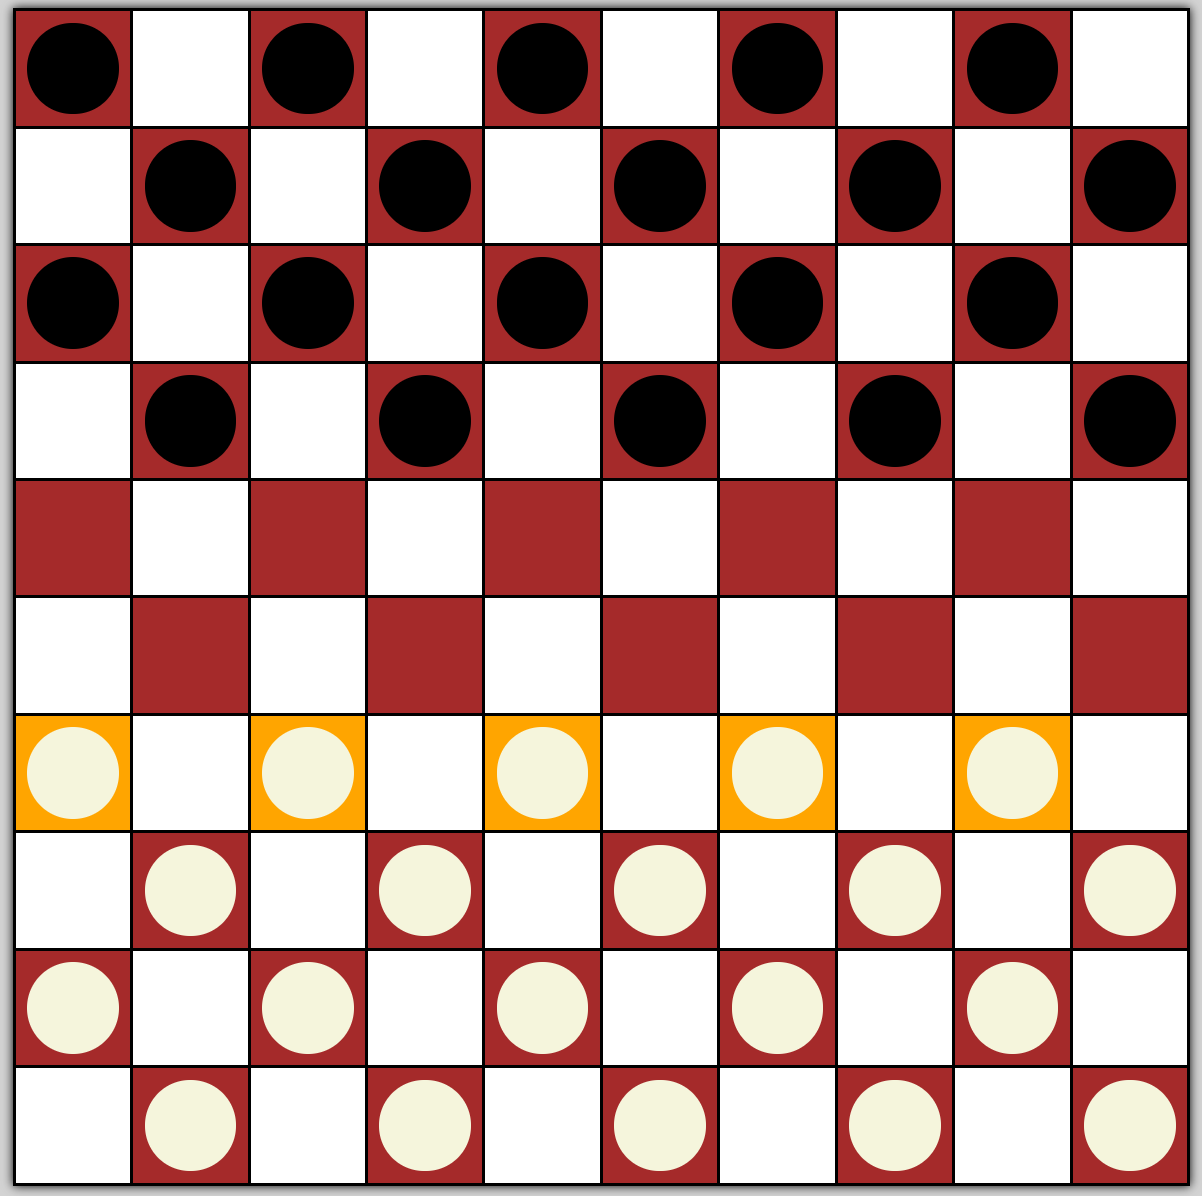
\includegraphics[width=0.5\linewidth]{pics/checkersboard.png}
	\captionof{figure}[DameSpielfeld]{ Das 10x10 Spielfeld aus der Anwendung }
	\label{fig:checkersboard}
\end{minipage}

\subsection{Minimax}
Der Minimax Algorithmus wird verwendet, um einen optimalen Spielzug in Spielen mit perfekter Information
zu finden. Allgemein wird eine Bewertungsfunktion verwendet, welche einen Zustand des Spieles bewertet und 
einen Integer Wert zurückgibt. Sehr niedrige Werte (negative) sind gut für Spieler A und sehr hohe Werte 
(positive) sehr gut für Spieler B. Um nun mehrere mögliche Zustände des Spieles zu berechnen und dann miteinander 
vergleichen zu können wird ein Suchbaum verwendet. siehe Abblidung \ref{fig:minimax}. Der Algorithmus beginnt bei den untersten Blättern und geht
nach oben bis zur Wurzel. Auf jeder Ebene wird versucht, je nach dem welcher Spieler an der Reihe ist, den Knoten zu
maximieren oder zu minimieren. Der Wert, welcher der Wurzel zugewiesen wird, ist auch der Spielzug, der als Nächstes
gespielt wird. 


\vspace{1em}
\begin{minipage}{\linewidth}
	\centering
	\includegraphics[width=0.5\linewidth]{pics/minimax.png}
	\captionof{figure}[minimax]{ Beispiel eines Minimax Suchbaumes }
	\label{fig:minimax}
\end{minipage}

\subsection{Alpha-Beta Pruning}
Das Alpha-Beta Pruning ist eine Optimierung zum Minimax Algorithmus. Die Idee des Algorithmus ist, 
dass manche Zweige des Suchbaums nicht untersucht werden müssen, da für den anderen Spieler diese
Züge nicht in Frage kommen. Hierbei ist $\alpha$ der Wert für den Spieler, für den die niedrigen Werte 
besser sind und $\beta$ für den anderen Spieler. Für jeden Knoten, je nach dem, ob er ein maximierender
oder ein minimierender Knoten ist, wird überprüft, ob ein Kind-Knoten, welcher einen neuen Wert
erhalten hat, nicht mehr vom Knoten beachtet werden muss. Z. B. ist der zu beachtende Knoten ein minimierender Knoten und 
hat aus seinem Linken Zweig eine 8 bekommen. Der rechte Kind-Knoten ist ein maximierender Knoten und
hat von seinen Kindern eine 9 bekommen, sodass es nun egal ist, welche weiteren Werte er von seinen anderen 
Kindern noch bekommt. Er wird seinen Wert nicht mehr unter 8 ändern, was zur Folge hat, dass der
rechte Zweig komplett ignoriert werden kann. 

\subsection{Monte Carlo Tree Search (MCTS)}
Der Monte Carlo Tree Search Algorithmus, ist ein heuristischer Algorithmus, bei welchem von einem
Zustand eines Spieles zufällig endlich viele Simulationen durchgeführt werden. Ein Vorteil des 
MCTS-Algorithmus gegenüber Minimax ist, dass erst am Ende eines Durchlaufs eine Bewertungsfunktion
benötigt wird. Allgemin besteht der Algorithmus aus vier Schritten:
\begin{itemize}
    \item \textit{Selektion}: Versucht wird, einen Zustand zu finden der noch erweiterbar ist, also
        einen Zustand zu finden, der kein Endzustand ist und noch nicht besuchte Züge hat.
    \item \textit{Expansion}: Der Spielbaum wird zufällig um einen noch nicht besuchten Zug erweitert.
    \item \textit{Simulation}: Von dem gewählten Knoten aus wird nun ein Spiel zufällig bis zum Ende 
        simuliert. 
    \item \textit{Backpropagation}: Das Ergebnis der Simulation wird den vorhergehenden Knoten mitgeteilt
        und diese werden mit diesem aktualisiert.
\end{itemize}
%todo -> UCT wert berechnung

\section{Anforderungsanalyse}
\subsection{Anwendungsszenario}
\subsection{Anforderungen an die Software}
\subsubsection{Nichtfunktionale Anforderungen}
\subsubsection{Funktionale Anforderungen}
\subsubsection{Zusammenfassung der Anforderungen}

\pagebreak
% ----------------------------------------------------------------------------------
% Kapitel: ???
% ----------------------------------------------------------------------------------

\section{Architektur}
\subsection{Überblick}
\subsection{Gameserver}
\subsection{Graphische Oberfläche}
\subsection{KI Client}

\section{Hardware}
\subsection{Raspberry Pi}
\subsection{Touch Monitor}

\section{Imlementierung}
\subsection{Eingesetzte Sofwarekomponenten}
\subsubsection{Programmiersprachen und Frameworks}
\subsubsection{Datentransferprotokolle}
\subsection{Gameserver}
\subsubsection{Netzwerkspezifikation des Gameservers}
\subsection{Graphische Oberfläche}
\subsubsection{Gegebene React Anwendung}
\subsubsection{Erweiterungen}
\subsection{KI Client}
\subsubsection{Vergleich der KI Algorithmen}

\section{Testing}
\subsection{Integrationstest}
\subsection{Ergebnisse}

\pagebreak
% ----------------------------------------------------------------------------------
% Kapitel: Fazit und Ausblick
% ----------------------------------------------------------------------------------
\section{Fazit und Ausblick}



\pagebreak
% ----------------------------------------------------------------------------------
% Kleine Einführung in LaTeX-Elemente
% ----------------------------------------------------------------------------------
%\section{\LaTeX-Elemente}
%Dieser Abschnitt beinhaltet lediglich einige Informationen über \LaTeX-Distributionen, Editoren und \LaTeX-Elemente, die Ihnen beim Einstieg in das \LaTeX-Textsatzsystem helfen sollen.
%
%\subsection{\LaTeX-Distributionen nach Betriebssystemen}
%
%\subsubsection{\LaTeX-Distributionen}
%Folgende Haupt-\LaTeX-Distributionen stehen Ihnen zur Verfügung:
%\begin{itemize}
%  \item Windows:\quad \texttt{MiKTeX}\quad Webseite:\quad\url{http://www.miktex.org}
%  \item Linux/Unix:\quad \texttt{TeX Live}\quad Webseite:\quad\url{http://tug.org/texlive/}
%  \item Mac OS:\quad \texttt{MacTeX}\quad Webseite:\quad\url{http://www.tug.org/mactex/}
%\end{itemize}
%
%\subsubsection{\LaTeX-Editoren}
%Auf folgenden Webseiten können Sie einige hilfreiche \LaTeX-Editoren finden:
%\begin{itemize}
%  \item Windows/Linux/Mac OS: \url{http://www.xm1math.net/texmaker/}
%  \item Windiws: \url{http://www.texniccenter.org/}
%  \item Mac OS: \url{http://pages.uoregon.edu/koch/texshop/}
%\end{itemize}
%
%Falls bei den oben genannten Editoren kein passender vorhanden war, findet sich auf Wikipedia eine Zusammenstellung vieler weiterer \LaTeX-Editoren:\\[1em]
%\hspace*{3cm}\url{https://en.wikipedia.org/wiki/Comparison_of_TeX_editors}
%
%
%\subsection{Bilder}
%Zum Einfügen eines Bildes, siehe Abbildung \ref{fig:reversi01}, werden die \texttt{minipage}-Umgebung und der Befehl \texttt{$\backslash$includegraphics} genutzt, da die Bilder so gut positioniert und einfach integriert und skaliert werden können.
%
%\vspace{1em}
%\begin{minipage}{\linewidth}
%	\centering
%	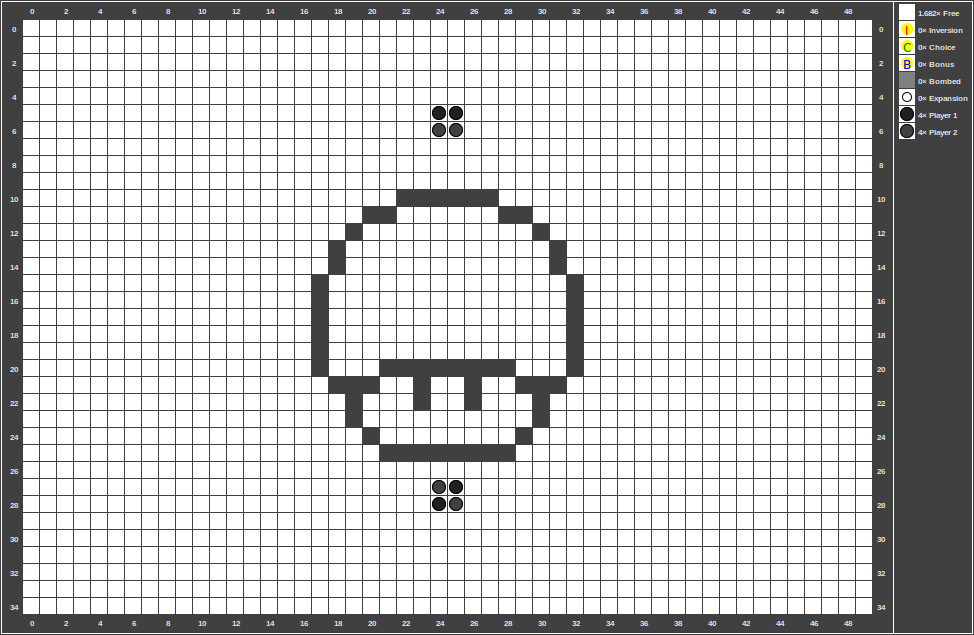
\includegraphics[width=0.5\linewidth]{pics/gamefield01.png}
%	\captionof{figure}[Spielfeld 01]{Unbespieltes Spielfeld\footnotemark }
%	\label{fig:reversi01}
%\end{minipage}
%\footnotetext{Diesem Spielfeld wurden noch keine Spieler zugewiesen (daher die dunklen Spielsteine)}
%
%Nachdem das Spielt gestartet wurde und beide Spielphasen durchlaufen wurden, siegt schließlich der Spieler mit der Farbe rot.
%
%\vspace{1em}
%\begin{minipage}{\linewidth}
%	\centering
%	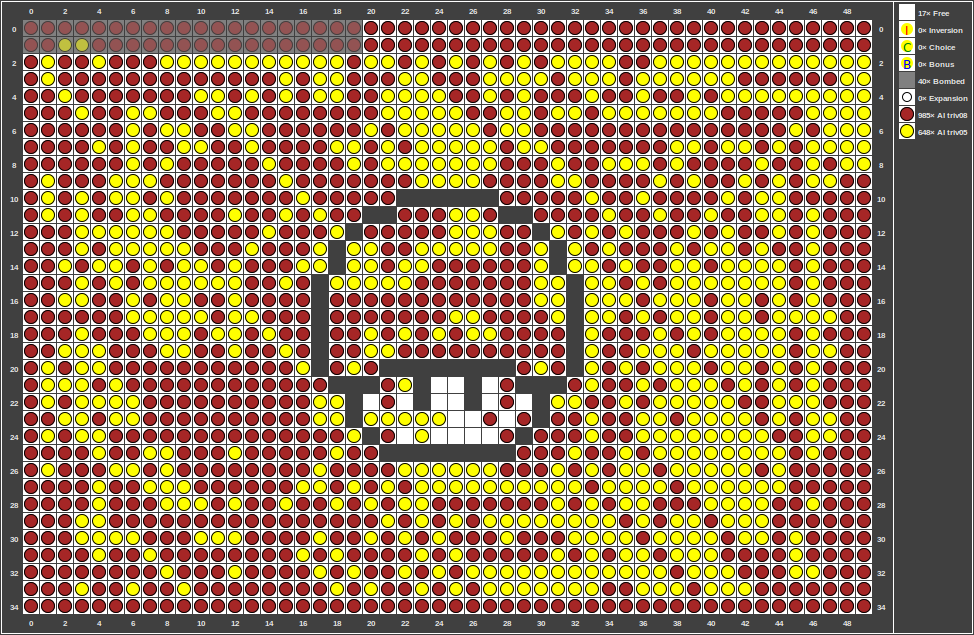
\includegraphics[width=0.5\linewidth]{pics/gamefield02.png}
%	\captionof{figure}[Spielfeld 02]{Finales Spielfeld\footnotemark }
%	\label{fig:reversi2}
%\end{minipage}
%\footnotetext{Das Spielfeld nach der Zug- und Bombenphase. Spieler rot gewinnt eindeutig.}
%
%\subsection{Tabellen}
%In diesem Abschnitt wird eine Tabelle (siehe Tabelle \ref{tab:beispiel}) dargestellt.
%
%\vspace{1em}
%\begin{table}[!h]
%	\centering
%	\begin{tabular}{|l|l|l|}
%		\hline
%		\textbf{Name} & \textbf{Name} & \textbf{Name}\\
%		\hline
%		1 & 2 & 3\\
%		\hline
%		4 & 5 & 6\\
%		\hline
%		7 & 8 & 9\\
%		\hline
%	\end{tabular}
%	\caption{Beispieltabelle}
%	\label{tab:beispiel}
%\end{table}
%
%
%\subsection{Auflistung}
%Für Auflistungen wird die \texttt{enumerate}- oder \texttt{itemize}-Umgebung genutzt.
%
%\begin{itemize}
%	\item Nur
%	\item ein
%	\item Beispiel.
%\end{itemize}
%
%\subsection{Listings}
%Zuletzt sehen Sie in Listing \ref{lst:maxTeilsumZweiD} ein Beispiel für das Einbinden von Quellcode mit Syntax-Highlighting.
%
%\vspace{1em}
%\lstinputlisting[caption=Brute Force-Ansatz für das MaxTeilsum2D-Problem, label=lst:maxTeilsumZweiD,basicstyle=\ttfamily\scriptsize]{code/maxTeilsum2DBruteForce.txt}
%
%\subsection{Selbstgestaltete Abbildungen}
%Mithilfe des Paketes \texttt{tikz} können sehr schöne Abbildungen (z.\,B.\ Automaten, Graphen etc.) direkt in \LaTeX generiert werden. Viele Beispiele dazu finden Sie auf folgender Webseite:\\[1em]
%\hspace*{3cm}\url{http://www.texample.net/tikz/}.
%
%\subsection{Tipps}
%Die Literaturreferenzen (Bücher, Paper und Journals) und Internetquellen (Webseiten, Blogs etc.) befinden sich in der Datei \textit{literatur.bib}. Eine Buch- und eine Online-Quelle sind beispielhaft eingefügt. [Vgl.\ \cite{buch}, \cite{mathcomm}]
%
%Literatur und Quellen werden in zwei getrennte Verzeichnisse aufgeteilt. Als Unterscheidungsmerkmal dient bei den Quellen der Zusatz: \texttt{keywords = \{online\}}.
%
%\pagebreak
%
%% ----------------------------------------------------------------------------------------------------------
%% Filter fuer Literatur und Quellen definieren
%% ----------------------------------------------------------------------------------------------------------
%
%\defbibheading{Literatur}{\section*{Literaturverzeichnis}} 
%\defbibheading{Quellen}{\section*{Quellenverzeichnis}} 
%  
%\defbibfilter{Literatur}{\not\keyword{online}} 
%\defbibfilter{Quellen}{\keyword{online}} 
%
%
%% ----------------------------------------------------------------------------------------------------------
%% Literatur
%% ----------------------------------------------------------------------------------------------------------
%\lhead{} 
%\rhead{Literaturverzeichnis} 
%
%\printbibliography[heading=Literatur,filter=Literatur] 
%
%\pagebreak
%
%
%% ---------------------------------------------------------------------------------------------------------- 
%% Quellen 
%% ---------------------------------------------------------------------------------------------------------- 
%\lhead{} 
%\rhead{Quellenverzeichnis} 
%
%\printbibliography[title = {Quellenverzeichnis}, heading=Quellen,filter=Quellen] 
%
%\pagebreak 
%
%% ----------------------------------------------------------------------------------------------------------
%% Anhang
%% ----------------------------------------------------------------------------------------------------------
%\pagenumbering{Roman}
%\setcounter{page}{1}
%\lhead{Anhang \thesection}
%
%\begin{appendix}
%\section*{Anhang}
%\phantomsection
%\addcontentsline{toc}{section}{Anhang}
%\addtocontents{toc}{\vspace{-0.5em}}
%
%Inhalt des beigefügten Datenträgers:
%\begin{itemize}
%  \item $\ldots$
%  \item $\ldots$
%\end{itemize}
%
%\section{Domändenmodell}
%Ein toller Anhang, der nicht nur als \glqq{}\emph{Müllhalde}\grqq{} genutzt wird, sondern in dem Bilder und Inhalte auch mit eigenen Worten erklärt werden und den man auch für sich alleine lesen kann. Es sollten auch Referenzen auf die zugehörige ausführliche Behandlung im Hauptteil inklusive Seitenangabe mit $\backslash$\texttt{pageref} gegeben werden.
%
%\subsection*{Screenshot}
%\label{app:screenshot}
%Unterkategorie, die nicht im Inhaltsverzeichnis auftaucht.
%
%\end{appendix}
%
%
%\pagebreak
%
%
%
%
\end{document}
%